\chapter{Electromagnetic Worldlines - Numerical Methods and Results}
\label{ch:numerical}

The ultimate goal of this project is to build a general numerical method. In order to test results 
it is necessary to test smaller cases carefully first.  Despite the emphasis on planar geometries,
we have tried to develop methods that would be well suited to more complicated geometries,
and test them in the simple geometry.  In this case we can carefully test their convergence properties
as the path resolution is increased.  

Even in a planar geometry we have had to develop an array of tools to make the worldline methods tractable.
The TM polarization is by far the hardest to deal with, and has prompted most of these developments.
The same developments can be used to enhance the TE polarization, as well as existing Dirichlet
worldline methods.

We will discuss techniques path construction, Monte Carlo sampling of the path starting points $x_0$
and path-time $\cT$.  In the case of the TE polarization, these are all quite straightforward.  
The TM polarization displays large numerical fluctuations, which must be tempered by changing the methods
used to construct the paths.  The essence of these methods is importance sampling, beyond what is manifestly
obvious from the form of the path integral.    

The numerical results will be compared against the expected efficiencies $\eta(\chi)$ and $\gamma(\chi)$.
The worldline method tends to straightforwardly reproduce the expected distance dependence due to the
integration over $\cT$, as was briefly discussed in Sec.~\ref{sec:worldline_distance_dep}. 
That is still true within the for electromagnetic worldlines. 
All of the simulations are carried out for a fixed $\chi$ in the far-field limit, but we will discuss how
to generalize the simulations to allow dispersion.  
The computations at fixed $\chi$ are useful indicators for how the full dispersion simulations.
In the Casimir effect, each frequency contributes independently, so for a particular frequency $\chi(i\omega)$
is effectively constant.  Since $\chi(i\omega)$ is a positive real constant, that diverges in some cases
(such as metals), it is necessary to see how the worldline algorithm performs across a whole range of susceptibilities.

The numerical results on the TE Casimir energies were published in Ref.~\cite{Mackrory2016}.

\section{TE Casimir Numerics}

In this section we will discuss numerically simulating the TE Casimir and Casimir--Polder energies 
from the worldline expressions in Eqs.~(\ref{eq:TE_Casimir}) and (\ref{eq:TE_Casimir_Polder}).
We will first discuss path generation, sampling starting positions $\vect{x}_0$ and path-times $\cT$,
and evaluating the dielectric path-average $\langle \epsr\rangle$.  % Despite working with expressions adapted to planar
% media, we will endeavour to develop general purpose numerical methods that would work in more general
% geometries.  

\subsection{Path generation}

The principal element of the worldline method is evaluating a potential along an ensemble of Gaussian
paths.  This allows the $N$-dimensional integral over positions to be efficiently evaluated in a 
Monte Carlo fashion via $N_p$ sample paths.
It is of primary importance to be able to efficiently generate these Gaussian sample paths. 

\subsubsection{Open Brownian Bridges: V-loop construction}

The v-loop algorithm is derived by decoupling the product of $N$ Gaussian probability densities 
into $N-1$ independent Gaussian deviates~\cite{Gies2003}.
Since we will need to construct open and closed Brownian bridges of fixed length $N$, we will derive the v-loop algorithm
for open paths, as closed paths are a special case of open paths.  

Consider a Gaussian density of $N$ steps in one dimension, where the end points $x_0$ and $x_N$ 
are fixed:
\begin{equation}
  P(x_1,\ldots,x_{N-1}) = (2\pi\Delta\cT)^{-N/2}\exp\left[-\sum_{j=0}^{N-1}\frac{(x_{j+1}-x_j)^2}{2\Delta\cT}\right].
  \label{eq:Gaussian_distrib}
\end{equation}
It is convenient to define a shifted, normalized variable $y_k = (x_k-x_0)/\sqrt{\Delta \cT}$.
The exponent for the product of coupled Gaussians is
\begin{equation}
X = \frac{y_1^2}{2}+\frac{(y_2-y_1)^2}{2}+\cdots+\frac{(y_{N-1}-y_{N-2})^2}{2}+\frac{(\Delta x-y_{N-1})^2}{2},
\label{eq:Xexp}
\end{equation}
where $\Delta x :=(x_N-x_0)/\sqrt{\Delta \cT}$.  
The exponent~(\ref{eq:Xexp}) can be decoupled by completing the square repeatedly.
The process starts at one end of the path $y_{N-1}$.  It is convenient to
introduce a variance $\sigma^2_{N-1}=1$ as a bookkeeping device.
It is possible to quickly develop recursion relations for how the resulting means and variance scale.  
\begin{align}
  & \frac{(y_{N-1}-\Delta x)^2}{2\sigma_{N-1}^2}+\frac{(y_{N-1}-y_{N-2})^2}{2} \nonumber \\
  &= \frac{\sigma^2_{N-1}+1}{2\sigma_{N-1}^2}
  \left(y_{N-1} - \frac{\sigma_{N-1}^2y_{N-2}+\Delta x}{\sigma_{N-1}^2+1}\right)^2 + \frac{(y_{N-2}-\Delta x)^2}{2(\sigma^2_{N-1}+1)}
  % &= \frac{1}{2c_{N-1}}
  % \left(y_{N-1} - c_{N-1}y_{N-2}-\frac{\Delta x}{\sigma_{N-1}^2+1}\right)^2 + \frac{(y_{N-2}-\Delta x)^2}{2(\sigma^2_{N-1}+1)}\\
\end{align}
where $\sigma_{N-2}:=\sigma_{N-1}+1$, and $c_{N-1} = \sigma_{N-1}^2/(\sigma_{N-1}^2+1)$.
After each completion of the square $\sigma_{N-j}\rightarrow \sigma_{N-j+1}+1$.  After repeating the process $N-1$ times
the exponent is 
\begin{equation}
  X = \frac{\Delta x^2}{2N} + \sum_{j=1}^{N-1} \frac{z_j^2}{2},
\end{equation}
where 
\begin{equation}
  z_j = \frac{1}{2c_j}\left(y_j - c_jy_{j-1}-\frac{\Delta x}{N-j+1}\right)^2,\label{eq:zj}
\end{equation}
and 
\begin{equation}
  c_j = \frac{N-j}{N-j+1}.
\end{equation}
The $z_j$ are decoupled standard normal variables.  Once the $z_j$ have been sampled the 
transformation (\ref{eq:zj}) can be inverted to find the path,
\begin{equation}
  x_k = x_0 + \frac{x_N-x_0}{N-k+1}+c_kx_{k-1} + \sqrt{c_k\Delta\cT}z_k.\label{eq:open_vloop}
\end{equation}
\comment{double check counting?}
There is then an remaining normalization factor of $e^{-(x_N-x_0)^2/(2\cT)}/\sqrt{2\pi\cT}$,  
which accounts for the Jacobian $\prod_{j}c_j=N^{-1}$ from changing variable.
This normalization is also the normalization factor derived in Eq.~\ref{eq:Gaussian_normalization}.
An integral against the probability density~(\ref{eq:Gaussian_distrib}) could be evaluated as follows,
\begin{equation}
  I = \int \prod_{j=1}^{N-1}dx_j P(x_1,\ldots,x_{N-1})f(x_1,\ldots,x_N)
  = \frac{e^{-\frac{(x_1-x_N)^2}{2\cT}}}{\sqrt{2\pi \cT}}\dlangle f\drangle_{x(t)},
\end{equation}
where the ensemble average is taken over open Brownian bridges betwen $x_0$ and $x_N$.
The limit of closed paths can be easily taken by setting $x_N-x_0=0$.
The v-loop construction is also straightforwardlygeneralized to vector Brownian bridges.  
This procedure allows the generation of a unit loop for $\cT=1$, which can then be integrated over
multiple starting points $x_0$ and total path-times $\cT$.  A closed unit Brownian bridge can be constructed 
as
\begin{equation}
  B_k = c_kB_{k-1} + \sqrt{\frac{c_k}{N}}z_k.\label{eq:unit_vloop}
\end{equation}
A shifted, scaled Brownian bridge can then be constructed as
\begin{equation}
  x_k = x_0 + \sqrt{\cT} B_k.
\end{equation}

The original v-loop algorithm used centered paths, where the average position $\langle x\rangle$ is subtracted from the path~\cite{Gies2003}.
This requires first constructing the Brownian bridge, and then subtracting off the mean position.  
This is inconvenient if the path is being generated on the fly 
without storage, or if there are stochastic elements to path construction.    
In Casimir--Polder applications (or when computing the stress-energy tensor~\cite{Schafer2016}),
 it is better to consider paths emanating from a single point $\vect{x}_0$.
  The starting point corresponds to the atom's location, or the point where
the stress-energy tensor is being computed.  

\subsection{Monte-Carlo sampling}

To evaluate the Casimir energy it is necessary to integrate the results for a single path over all
starting points $\vect{x}_0$, path-times $\cT$, and average over an ensemble of paths.
% The rationale for also sampling over times is to allow further ensemble averaging over paths,
% and times. 
The original Gies\etal computations emphasized computing the total $\cT$ integral for each path~\cite{Gies2003}.
For Dirichlet worldlines, the path integrand is either zero or one based on whether the path intersects
all of the bodies.  This makes evaluating the integral a tractable problem, since 
it only requires finding the set of times $\{\cT_k\}$ when paths enter the body, and evaluating 
$\int_{\cT_0}^{\cT_1} d\cT\,\cT^{-(1+D/2)}$ during those  times the integral is nonzero.
For example, in their paper computing forces in a sphere-plane geometry Weber and Gies find analytical
expressions in terms of $\vect{x}_0$ and $\cT$ for when each random path will intersect both bodies~\cite{Weber2010}.
The remaining integrals over $\vect{x}_0$ and $\cT$ can be evaluated on a path-wise basis.

However, for the dielectric integrands that the TE and TM path integrals require, 
the integrand changes value based on how many points are inside the surface.  For a path of length $N$, this direct method would
require finding all $N$ intersection times and then evaluating the integrals.  
This becomes impractical for large $N$, as a large computational effort  must be expended on even a single path.  
This becomes even more burdensome once the integral over the starting position is accounted for.

Since the $N$-fold integral over positions is being handled in a Monte Carlo fashion, it makes sense to 
treat the remaining integrals over the starting position $\vect{x}_0$ and path-times $\cT$ in the same manner.
Each path can be evaluated for a single pair of $\vect{x}_0$ and $\cT$, where those are picked from suitable
distributions, governed by the form of the integral.  This is a form of importance sampling, which 
is a powerful tool for accelerating Monte Carlo numerical computations~\cite{Asmussen2007, Glasserman2004}.
This style of importance sampling goes beyond just using the Gaussian probability density to evaluate the 
spatial integrals over the intermediate positions $\vect{x}_k$.  In this case, the importance sampling
relies on knoweldge on which positions and times the most to the integral. 
This Monte Carlo sampling of $x_0$ and $\cT$ also extends the number of independent paths that can be averaged over, which 
is essential for good convergence.   

\subsubsection{Sampling Path-Times from a Power Law}

The simplest method of sampling path-times, is to exploit the presence of $\cT^{-(1+D/2)}$ in the integral.
For a particular path, the renormalized TE integrand is only non-zero after the path touches all of the bodies,
which occurs at some path-time $\cT_0$.\footnote{For a Brownian motion $\vect{x}(t)$,
the term ``first-touching time'' is reserved for the first time $t_0$ along a path that a Brownian bridge intersects a surface: $\vect{x}(t_0)=d$. 
This is distinct from the first path-time $\cT$ when any section of the scaled path intersects a surface.
}
For $\cT>T_0$,  the extent of the path grows as $\sqrt{\cT}$, so the integrand $(\langle\epsr\rangle^{-\alpha}-1)$ 
increases as more points enter the bodies.  
However, the $\cT^{-(1+D/2)}$ factor decreases the contributions from large path-times $\cT$.
These facts suggest sampling $\cT$ from a probability distribution 
\begin{equation}
  P(\cT;\cT_0,m)= \frac{(m-1) \cT_0^{m-1}}{\cT^m}\Theta(\cT-\cT_0),\label{eq:Tpower_law}
\end{equation}
where $m>1$ and $\cT_0>0$.  This requires being able to estimate the value of the first-contact time $\cT_0$.  
For the example of paths starting between parallel planes $\cT_0=\text{min}[\left(\frac{-d_1-x_0}{B_-}\right)^2,
\left(\frac{d_2-x_0}{B_+}\right)^2]$ where $d_1<x_0<d_2$, and $B_\pm$ are the maximum and minimum points
of the unit Brownian path.  The path-time $\cT_0$ is the lowest bound on when the path will touch the relevant bodies.
In computing Casimir interaction energies, the path must touch \emph{all} of the bodies, while in Casimir--Polder
calculations, the path must touch \emph{any} of the bodies to contribute.  

Samples from the distribution~(\ref{eq:Tpower_law}) can be generated by inverting the cumulative probability distribution.
(This sort of inversion is a general purpose method of generating random deviates from a distribution~\cite{NumRecipe,Devroye2003}.)
In this case, the inversion requires a solution $\cT$ to
\begin{equation}
  r=(m-1) \cT_0^{m-1}\int_{\cT_0}^\cT dt\, t^{-m}
\end{equation}
where $r\in [0,1]$ is a uniform random number and $\cT$ is the desired deviate.    
This can be easily solved, with the result that
\begin{align}
%  r&=(m-1) \cT_0^{m-1}\frac{1}{m-1}\left(\frac{1}{\cT_0^{m-1}}-\frac{1}{\cT^{m-1}}\right)\\
%  \left(\frac{\cT_0}{\cT}\right)^{m-1}&= (1-r)\\
 \cT= \frac{\cT_0}{(1-r)^{1/(m-1)}}.
\end{align}
The lower-bound $\cT_0$ can be easily found in simple geometries on a path-wise basis. Deviates
$\cT$ can then be generated for each path, where each path is then guaranteed to contribute.  

In a more complicated arrangement of bodies, the lower-bound $\cT_0$ could be found via root-finding,
to find the minimum path-time that the path touches all of the relevant bodies.  It is important for 
$\cT_0$ to be a lower bound on the first time the integrand is nonzero, otherwise this method will miss 
part of the integral.  However, $\cT_0$ should not be set too low, as otherwise numerous samples will
be made which generates paths that are too small to contribute.  

\subsubsection{Sampling Starting Positions}

The integral over the starting point $x_0$ can also be evaluated in Monte-Carlo fashion by exploiting some knowledge 
about the form of the integrand.  
For points $x$ far from all bodies located around the origin, the expected minimum path-time when the integrand is nonzero 
is $\cT_0\sim x^2$.
If the extent of the finite bodies is $d_{\text{max}}$, then there is also a maximum time $\cT_1$ for when the path is so large 
that it does not intersect the bodies anymore (this may be infinite in some geometries).
In that case, and approximating the integrand $(\langle\epsr\rangle^{-1}-1$ by its strong-coupling limit,
the path-time integral is approximately 
\begin{equation}
  \int_{\cT_0}^{\cT_1} \frac{d\cT }{\cT^{1+D/2}} = \frac{1}{x^{D}}-\frac{1}{d_{\text{max}}^D}.
\end{equation}
This suggests that the contribution from points far from the bodies scales at most as $x^{-D}$.  
In between the bodies, the contribution from each starting position is roughly uniform, since each path must have sufficient extent
to touch all bodies.  
This occurs for times $\cT\sim d_0^2$, where $d_0$ is the separation between bodies.    
In a one-dimensional geometry, embedded in a four-dimensional space-time, 
these considerations suggest sampling from 
\begin{equation}
  P_x(x;d_0):= \frac{3}{8d_0}\left\{ \begin{array}{cc}
    1  & |x|<d_0\\
    \dfrac{d^4_0}{|x|^4} & |x|>d_0
  \end{array}
\right.\label{eq:xPower_law}.
\end{equation}
This reasoning can be easily extended to higher dimensional problems,
where a sphere of radius $d_0$ should bound all of the interfaces between the bodies.
Outside of that sphere, the sampling would again fall off as $|x|^D$.  
While it may be possible to develop sampling procedures better suited to a particular geometry, 
this provides a general purpose way of sampling the starting points for Casimir worldline path integrals.

\subsubsection{Evaluating the Dielectric Path Average}

Once a path is constructed, the rest of the path integral integrand can be sampled along that path.
For example, the path average of the dielectric can be evaluated as 
\begin{equation}
  \langle\epsr\rangle = \frac{1}{N}\sum_{k=1}^N\epsr(x_k).
\end{equation}
This corresponds to the trapezoidal rule for evaluating the path-average, 
\begin{equation}
  \langle\epsr\rangle = \frac{1}{\cT}\sum_{k=0}^{N-1}\int\limits_{k\Delta\cT}^{(k+1)\Delta\cT} dt'\, \epsr[x(t')]
  \approx = \frac{\Delta \cT}{N}\sum_{k=0}^{N-1}\frac{\epsr(x_k)+\epsr(x_{k+1})}{2}=\frac{1}{N}\sum_{k=1}^N\epsr(x_k)
\end{equation}
where the trapezoidal rule $\int_a^b dx\,f(x)=(b-a)[f(a)+f(b)]/2$, was used for each time integral.
As discussed in \S 5.C.3 of Ref.~\cite{Mackrory2016}, the trapezoidal rule outperforms some improved methods.  
For example, in cases where $x_k$ and $x_{k+1}$ straddle a surface at $d$, the integral could be 
weighted by the fraction of the path increment inside the surface, $(x_{k+1}-d)/(x_{k+1}-x_k)$.
This reduces the contribution from path increments where one point just enters the surface.  
Unfortunately, this does not fix an opposing error: what about paths that come close to the surface but just 
miss it?  There is some finite probability that a sub-path between $x_k$ and $x_{k+1}$ would have entered the body, and given a greater 
contribution.  Since the reduction of the contribution is not offset, this more advanced method actually
fares worse than the straightforward trapezoidal method. 

\subsection{TE Casimir  and Casimir--Polder Energies - Plane-Plane}

These methods can be applied to computing the TE Casimir and Casimir--Polder energies.  
As a first step, let us consider the Casimir--Energy for an atom interacting with a dielectric half-space 
in the zero temperature, far-field limit.  The atom is located at the origin, with a dielectric half-space 
a distance $d$ away with a constant susceptibility $\chi$.

Fig.~\ref{fig:eff_TE_atom_wall} shows the numerical results for evaluating the TE Casimir--Polder path integral~(\ref{eq:TE_Casimir_Polder})
at a range of $\chi$.  
The TE Casimir--Polder energy is calculated numerically by evaluating
\begin{align}
  V\supTE\subCP-V_0 %&= -\frac{\hbar c\alpha_0}{8\pi^2}\biggdlangle \int_0^\infty\frac{d\cT}{\cT^{3}}\big(\langle \epsr\rangle^{-3/2}-1)  \biggdrangle \nonumber\\
  &=\biggdlangle \frac{\hbar c\alpha_0}{8\pi^2} \frac{1}{2\cT_0^{2}}\left(\frac{1}{\langle\epsr(x_k)\rangle^{-1/2}}-1\right) 
    \biggdrangle_{\vect{x}_k,\cT},\label{eq:TE_CP_num}
\end{align}
where $\dlangle \cdots\drangle_{\vect{x}_k,\cT}$ denotes an ensemble average over discrete Brownian bridges,
and times $\cT$.  
One dimensional Brownian bridges are constructed using the v-loop algorithm~(\ref{eq:unit_vloop}).
The minimum path-time $\cT_0$ is determined on a path-wise basis, based on solving $\sqrt{\cT_0}\text{max}(B_k)=d$.
The path-time is sampled for each path from Eq.~(\ref{eq:Tpower_law}), with $m=1+D/2=3$.
The path is then scaled, $x_k = \sqrt{\cT}B_k$, and the trapezoidal method is used to evaluate $\langle\epsr\rangle$
around each path.  The sojourn time per path $\langle\Theta(x-d)\rangle$ can be estimated once per path,
and then multiple $\chi$ can be computed at once using $\langle \epsr\rangle = 1+\chi\langle\Theta(x-d)\rangle$.
The results are then accumulated over many paths and times.  
The numerically calculated efficiency $\eta(\chi)$ is found by dividing the numerical results by the perfect-conductor result,
which cancels out the leading constants and the $d^{-4}$ distance dependence.

% As the results show, the agreement with between the numerical results
% and the analytical expression is excellent.  A more careful discussion of the numerical error is 
% deferred to Sec.~\ref{sec:TE_convergence}.
\begin{figure}
  \centering
 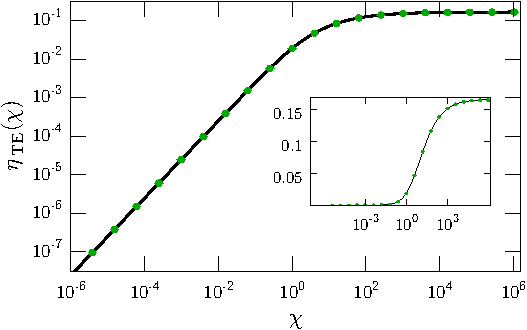
\includegraphics[width=0.8\textwidth]{fig/temp/eff_TE_atom_wall}
  \caption[Planar Casimir--Polder TE energy as function of $\chi$]
  {Planar Casimir--Polder TE energy as function of susceptibility $\chi$.  
    The simulations used $10^8$ paths, with $10^4$ points per path.
    Results for each $\chi$ were computed using the same ensemble of paths.
    The solid black line is the analytical result~(\ref{eq:etaTE}), and the points are the numerical
    values computed using Eq.~(\ref{eq:TE_CP_num}).
    (The inset is same data on a linear vertical scale.)
    }
  \label{fig:eff_TE_atom_wall}
\end{figure}

% Each path was generated with the v-loop algorithm~(\ref{eq:vloop}). 
% A single path-time $\cT$ was sampled for each path by sampling from Eq.~\ref{eq:Tpower_law}, 
% where $\cT_0$ is the smallest path-time that the part starting at $x_0$ would contact a planar surface a distance $d$ 
% away.  For TE integrands, a whole range of $\chi$ can be evaluated in parallel for a single path since 
% $\langle \epsr\rangle = 1+\chi\langle\Theta(x-d)\rangle$.  The path-averaged occupation time can be computed once for a 
% given path, and re-used to compute the Casimir--Polder energy for various $\chi$.  

% The numerically sampled values agree well with the analytical result for the 
% efficiency $\eta(\chi)$.  The efficiency is the ratio of the TE Casimir--Polder energy between an atom and a dielectric 
% to the total Casimir--Polder energy for an atom and a perfectly conducting plate.  This approaches $1/6$ in the 
% strong-coupling limit---the remainder of the Casimir--Polder energy is provided by the TM polarization, which
% will be discussed further in Sec.~\ref{sec:TM_numerics}.

\begin{figure}
  \centering
  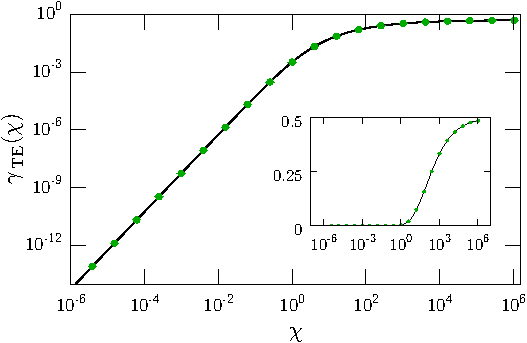
\includegraphics[width=0.8\textwidth]{fig/temp/eff_TE_2wall}
  \caption[Planar TE Casimir energy as function of $\chi$.]{
    Numerically calculated planar TE Casimir energy as function of $\chi$.
    The black lines show the analytical solution~(\ref{eq:gammaTE}), and the points show the numerical
    estimates.
    The simulations used $10^8$ paths, with $10^4$ points per path.  All values of $\chi$ were computed in parallel
    using the same ensemble of paths.
    (Inset is same data on a linear vertical scale.)}
  \label{fig:eff_TE_2wall}
\end{figure}

Fig.~\ref{fig:eff_TE_2wall} shows the numerically computed Casimir energy between two planar dielectric interfaces
a distance $d$ apart, with dielectric function $\epsr(x) = 1+\chi\Theta(-x+d/2)+\chi\Theta(x-d/2)$.  
This is computed numerically by evaluating
\begin{align}
  E\supTE\subCP-E_0 
  &=\biggdlangle \frac{\hbar c\alpha_0}{8\pi^2} \frac{1}{2\cT_0^{2}P_x(x_0)}
  \left(1+\frac{1}{\langle\epsrab(x_k)\rangle^{3/2}}-\frac{1}{\langle\epsra(x_k)\rangle^{3/2}}-\frac{1}{\langle\epsrb(x_k)\rangle^{3/2}}\right) \biggdrangle_{x_k,\cT,x_0},\label{eq:TE_Casimir_num}
\end{align}
The same procedure is similarto the one used for Casimir--Polder energies.  However, 
in this case there is an additional ensemble average over path starting position $\vect{x}_0$.
The starting positions are sampled from Eq.~(\ref{eq:xPower_law}), with $d_0=d$, 
which is twice the size of the region between the interfaces.  
In this case it is also necessary to keep track of $\langle \theta(x-d_2)\rangle$ and $\langle \theta(d_1-x)\rangle$.
The dielectric path average and the renormalized worldline integrand can also be quickly computed for multiple $\chi$.
One upshot of Monte Carlo sampling of positions is that this is \emph{much} faster than directly evaluating 
the position and path-time integrals on a path-wise basis.  In fact, evaluating the Casimir energy takes 
roughly the same time as the Casimir--Polder energy.  

\subsubsection{Scaling with N}
\label{sec:TE_convergence}
Some interesting scaling behaviour was found by examining the relative error between the numerical 
estimates and the exact analytical value.  
In this case the primary systematic error is due to the discretization of the path.
The path integral was derived under the assumption that $N\rightarrow\infty$, while the numerical
simulations use a discrete path with a finite $N$.  
There is an additional random error associated with the finite number of paths.   However, for $N_{\text{path}}$ paths,
this error scales as $N_{\text{path}}^{-1/2}$, as is typical for Monte Carlo sampling error.  This is what provides
the noise floor in Fig.~\ref{fig:conv_atom} and \ref{fig:conv_wall}.

\begin{figure}
  \centering
  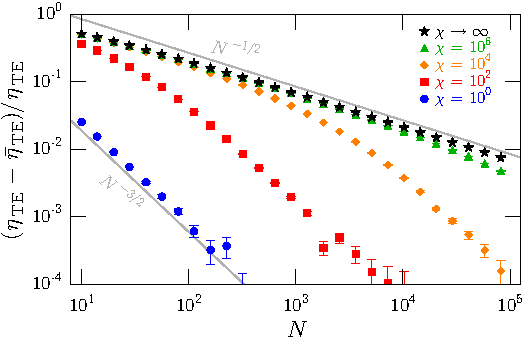
\includegraphics[width=0.8\textwidth]{fig/temp/conv_TEatomN3}
  \caption[Convergence of planar TE Casimir--Polder energy  as function of $N$.  ]{
    Convergence of planar TE Casimir--Polder energy as function of $N$.  
    Different values of $\chi$ use the same ensemble of paths.
    Simulations used $10^8$ paths, which sets the $10^{-4}$ noise floor.}
  \label{fig:conv_atom}
\end{figure}

\begin{figure}
  \centering
  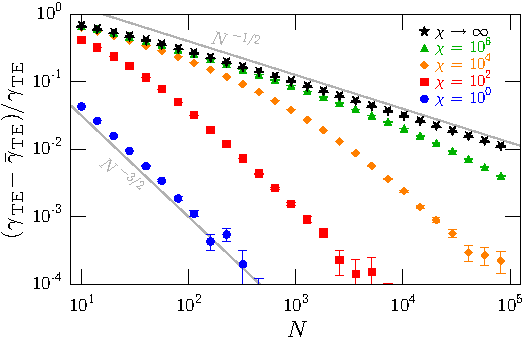
\includegraphics[width=0.8\textwidth]{fig/temp/conv_TE2wallN3}
  \caption[Convergence planar TE Casimir energy as function of $N$ for various $\chi$.]{
    Convergence planar TE Casimir energy as function of $N$ for various $\chi$, using the same ensemble of paths for all $\chi$.
    Simulations used $10^8$ paths, which sets the $10^{-4}$ noise floor.}
  \label{fig:conv_wall}
\end{figure}

As the path resolution $N$ varies for fixed $\chi$, the error shows two different scaling behaviours.  
In Ref.~\cite{Mackrory2016}, some arguments are given to explain this scaling, which will not be repeated here,
but we will explain the basic reasoning.  The numerical computations use discrete paths, 
while the path integral assumes $N$ is arbitrarily large.  Thus the paths considered by the path integral
have arbitrarily fine structure, with a non-zero probability to touch, or enter the dielectric body.
The discrete paths used in the numerical method miss those contributions.  

In the weak-coupling limit $\chi/N\ll 1$, the numerical estimate is dominated by accurately estimating the sojourn
time $\langle\theta\rangle$ for a given path.  Further increasing $N$ increases the accuracy of this 
estimate and renormalized integrand.  The $N^{-3/2}$ scaling can be estimated by integrating up the probability for a nonzero sojourn time
from each increment.  

In the strong-coupling limit $\chi/N\gg 1$, the integrand immediately saturates, and returns one.
Thus the dominant error comes from underestimating the time that this occurs.  The error scaling
is estimated by integrating up the probability that a continous path \emph{did} touch the surface
prior to the estimated first contact time.  This leads to a $N^{-1/2}$ scaling.

For a fixed $\chi$, the transition between both behaviours is observed at $N\sim\chi$. 
In the strict $\chi\rightarrow\infty$ Dirichlet limit, the numerical results and scaling 
arguments suggests that the numerical error will always scaled as $N^{-1/2}$.  However, for a finite
$\chi$ there is always such an $N$, although that $N$ grows linearly as the susceptibility increases.  

\section{TM Casimir Numerics}
\label{sec:TM_numerics}

Numerically calculating the Casimir energy due to the TM polarization is much harder than the TE case. 
This is due to the TM potential.
Even after regularization, and analytical path averaging, is still challenging to handle numerically.
We will develop a number of techniques to temper these difficulties that should have applications for more general Casimir worldlines.

The most daunting feature of the TM Casimir worldline is the singular TM potential.
 A closed form solution for the TM potential $V\subTM$ at a single planar boundary was found in Ch.~\ref{ch:feynman_kac}.
The ensemble averaged solution between points $x_k$ and $x_{k+1}$ in time $t$ is 
\begin{align}
  v_k(x_k,x_{k+1}):=\,&  \Bigdlangle e^{-\int_0^t dt'\, V\subTM(x-d)}\Bigdrangle_{x_k\rightarrow x_{k+1}} \\
   =\,& \Theta[X_{k,k+1}]\big[1 + \sgn(d-x_k)e^{-2X_{k,k+1}/t}\tanh\Xi\big]
  +\Theta[-X_{k,k+1}]\sech\Xi,
   \label{eq:TM_pot}
\end{align}
where $X_{k,k+1}:=(d-x_k)(d-x_{k+1})$.
This ensemble-averaged solution was plotted in Fig.~\ref{fig:TMpot}, 
for starting points on either side of the interface at various values of $\Xi$.
The solution is between zero and one for paths that start inside a body, or cross an interface.
For paths starting outside a body, the solution is between one and two.  The extreme values of zero and 
two only appear in the strong-coupling limit close to the suface.

This solution can be used in the path integral by identifying averages of sub-paths
between discrete points with the analytical solutions.
The path-averaged exponential potential can be split into many steps between $\vect{x}_k$ and $\vect{x}_{k+1}$
at times $\cT_k$ and $\cT_{k+1}$.  Each exponential potential can be averaged against all possible sub-paths
between these points.  
\begin{align}
  \biggdlangle \frac{e^{-\cT\langle V\rangle}}{\langle\epsr\rangle^{1/2}}\biggdrangle = &
  \biggdlangle \frac{1}{\langle \epsr\rangle^{1/2}}\prod_{k=1}^N
  \bigglinklangle \exp\left(-\int_{\cT_k}^{\cT_{k+1}} dt\, V[x(t)]\right)\bigglinkrangle_{x_k\rightarrow x_{k+1}}
    \biggdrangle\\
 =& \biggdlangle \frac{1}{\langle \epsr\rangle^{1/2}}\prod_{k=1}^N  v_{k,k+1}    \biggdrangle
  \end{align}
  It is not strictly necessary to include the dielectric average in the averaging over
sub-paths, since the dielectric is a much smoother function.  % Taking the dielectric into the average of sub-paths would lead to 
% even better results, but those analytical solutions are difficult to calculate.
The integrand can be built up even for a discrete Brownian bridge of length $N$, 
by multiplying the appropriate TM potential terms~(\ref{eq:TM_pot}) along the path, and then dividing
by the path-average of the dielectric $\langle\epsr\rangle$.  

% This notion of replacing a singular potential with its ensemble averaged value between two end points
% is a powerful one.  This technique also offers an improvement on the accuracy for Dirichlet boundary conditions,
% and which will be discussed further in Secs.~\ref{sec:general_gradient} and \ref{sec:accel_converge}.

\subsection{Scaling of Averaged TM Potential with Path Resolution}

Even after regularization, and ensemble averaging the TM potential is still difficult to handle.  
The numerical properties of the solution can be examined by considering a simplified path integral
that only includes a single TM potential a distance $d$ away,
\begin{align}
  I=\dlangle e^{-\int_0^\cT dt\,\VTM[x(t)]}\drangle_{\vect{x}(t)} =\,& \Biggdlangle \prod_{k=0}^{N-1}
  \bigglinklangle  e^{-\int_0^{\Delta \cT} dt\,\VTM[x(t)]}\bigglinkrangle_{x_k\rightarrow x_{k+1}}\Biggdrangle_{\vect{x}_k}\\
=\,&\Biggdlangle \prod_{k=0}^{N-1}
  v_{k,k+1}\Biggdrangle_{\vect{x}_k}.
\end{align}
The left-hand ensemble average is over continuous Brownian bridges, whereas the second ensemble
average runs over discrete Brownian bridges (and averaging over continuous sub-paths indicated by $\linklangle\cdots\linkrangle$).
In this case, the exact value of the integral is just the TM potential solution Eq.~\ref{eq:TM_pot},
for $x_k=x_{k+1}=x_0$.  The right hand side can be computed numerically, its scaling with $N$ can be
examined.

Fig.~\ref{fig:TM_histogram} shows a histogram of numerical estimated values for closed Brownian paths 
interacting with the TM potential.  Each Brownian path is generated via the v-loop algorithm~(\ref{eq:unit_vloop}),
and scaled by $\sqrt{\cT}$.  The total contribution from each path is the product of the TM solutions~(\ref{eq:TM_pot}) for every
step along the path.
The direct estimate of the TM potential shows a wide spread of values.
 Most paths return values close to zero, while a few rare paths return very large values.  
This suggests that the plain Gaussian paths 
are poorly suited to this problem, and that the path generation scheme should be modified.
Given a large enough ensemble, this eventually converges to the right answer, but it displays
unacceptably large numerical fluctuations.  

\begin{figure}
  \centering
  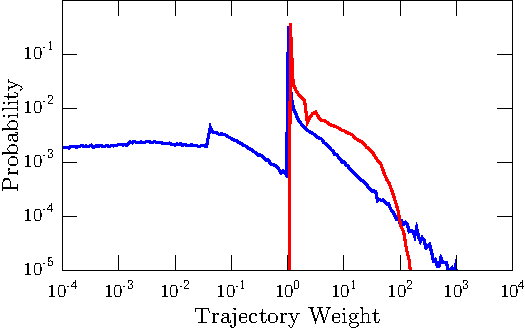
\includegraphics[width=0.8\textwidth]{fig/numerics/TM_normhist}
  \caption[Histogram of Accumulated Numerical TM Estimates]
  {Histogram of accumulated numerical TM estimates, for raw Gaussian (blue) and birth-death Gaussian (red).
    Simulations used $10^6$ paths, with $N=100$ points per path, $\chi=100$, $d=1,T=1.$
  The raw Gaussian distribution extends off to negative infinity, while the birth-death distribution has trunctated peak at zero weight.}
\label{fig:TM_histogram}
\end{figure}

\subsubsection{TM-Gaussian paths}

\begin{figure}
  \centering
  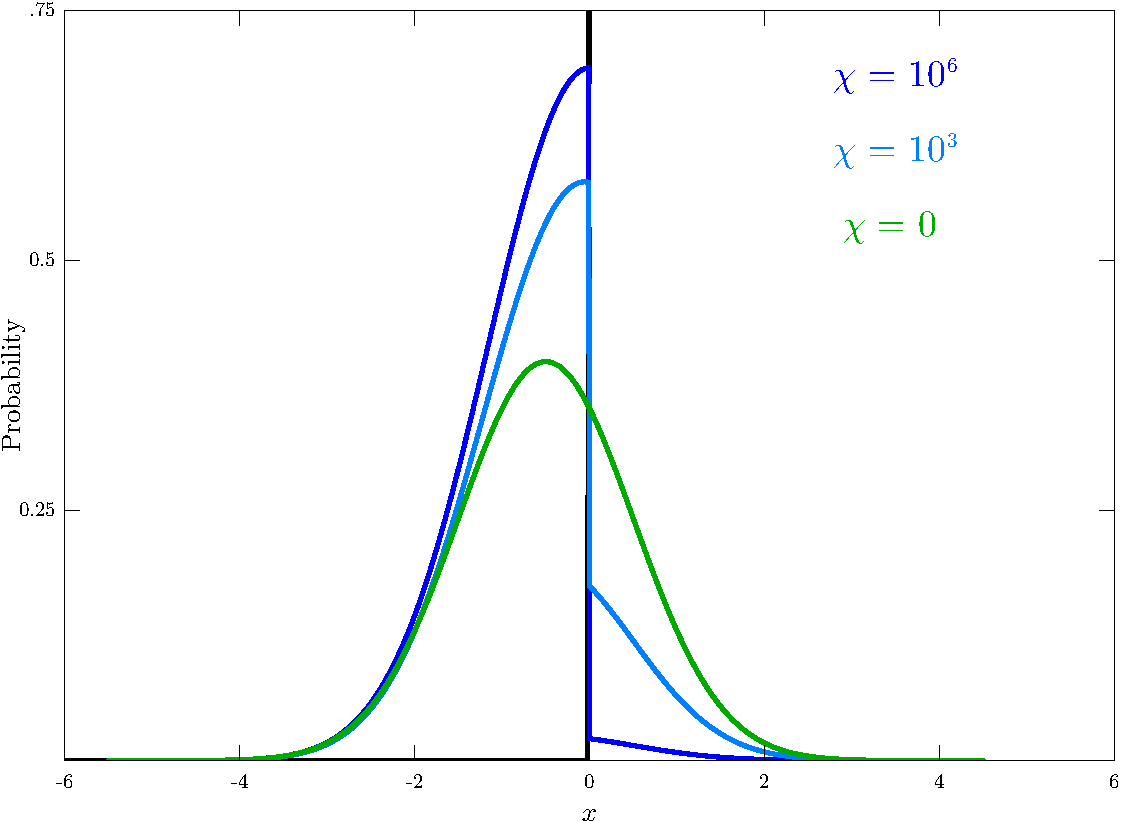
\includegraphics[width=0.8\textwidth]{fig/analytical/probTM}
  \caption[Combined TM Potential and Gaussian probability distribution.]{
    Combined TM-Gaussian probability distribution plotted for various $\chi$.
    Increment starting position is $x=-1$, and $\cT=1$.  The TM boundary is at the origin. }
\end{figure}

One possible solution to the fluctuations is to sample from a combination of a Gaussian
and the path-averaged exponential~(\ref{eq:TM_pot}) for the path increment.
In this case, the total probability distribution for the paths is 
\begin{align}
  P(x_1,\ldots ,x_{N-1}) = \prod_{k=0}^{N-1}\frac{e^{-(x_{k+1}-x_k)^2/(2\Delta\cT)}}{\sqrt{2\pi\Delta\cT}}
  \bigglinklangle e^{-\int_0^{\Delta \cT}dt\, \VTM}\bigglinkrangle_{x_k\rightarrow x_{k+1}}
\end{align}
In the same manner as the v-loops, the Gaussian probability distribution can be decoupled into a
set of random variables, where from Eq.~\ref{eq:open_vloop}, the argument of each of those Gaussians 
involves ${z_k = (x_k-c_{k}x_{k-1})/\sqrt{c_k\Delta \cT}}$.
\begin{align}
  P(x_1,\ldots ,x_{N-1}) = v_{N,N-1}\prod_{k=0}^{N-1}\cN_{k+1}^{-1}P\supTM_{k+1}(x_{k+1}),
\end{align}
where the new probability distribution for $x_k$ is 
\begin{align}
P\supTM_{k+1}(x_{k+1}):=\cN^{-1}_{k+1}\frac{e^{-(x_{k+1}-c_k x_k)^2/(2c_k\Delta\cT)}}{\sqrt{2\pi c_k\Delta\cT}}v_{k,k+1}(x_k,x_{k+1}),
  \end{align}
with normalization constant 
\begin{align}
  \cN_k=\int dy\, \frac{e^{-(y-c_k x_k)^2/(2c_k\Delta\cT)}}{\sqrt{2\pi c_k\Delta\cT}}v_{k,k+1}(x_k,y).
\end{align}
The crucial point is that the $P\supTM_{k}$ can be sampled from, accounting only for the present position. 
While the present position $x_k$ is still coupled to future positions via $v_{k+1,k}$, the sampling procedure ignores
that coupling and samples $x_k$ based solely on $P_k$.  
The probability distribution can be put into a convenient numerical form by completing the square to account
for $v_{k,k+1}$.  The resulting piecewise Gaussian probability distribution is 
\begin{align}
  P\supTM_{k+1}(x_{k+1})
 = \cN_k\left\{ \begin{array}{lc}
     \vspace{0.2cm}  \dfrac{e^{-(x_{k+1}-c_k x_k)^2/(2c_k \Delta\cT)}}{\sqrt{2\pi c_k \Delta\cT}} + \sgn(d-x_k)\dfrac{\tanh\Xi}{\sqrt{2\pi c_k \Delta\cT}} & \hspace{2cm}\\
    \vspace{0.2cm} \hspace{0.7cm}\times e^{-(x_{k+1}-c_k(2d-x_k))^2/(2c_k \Delta\cT)} e^{-2(1-c_k)d(d-x_k)/\Delta\cT} &  X_{k,k+1}>0\\
\dfrac{\sech \Xi}{\sqrt{2\pi c_k \Delta\cT}}e^{-\frac{(x_{k+1}-c_k x_k)^2}{2c_k \Delta\cT}}  &  X_{k,k+1}<0\,,\\
\end{array}
\right.\label{eq:PTM_k}
\end{align}
where we previously defined $X_{k,k+1}=(d-x_k)(d-x_{k+1})$.  
The normalization constant integral can be evaluated in two parts $\cN_k=\cN_k^{\text{C}}+\cN_k^{\text{NC}}$, 
a crossing term $\cN_k^{\text{C}}$ for $X_{k,k+1}<0$,  and non-crossing term $\cN_k^{\text{NC}}$ for $X_{k,k+1}>0$,
 with the result
\begin{align}
  \cN_k^{\text{C}}=\,& \frac{1}{2}\left[1+\sgn(d-x_k)\, \erf\!\left(\frac{d-c_k x_k}{\sqrt{2 c_k \Delta\cT}}\right)\right] \nonumber\\
  &+\sgn(d-x_k) \frac{\tanh\Xi}{2}\left[1+ \sgn(d-x_k)\,\erf\!\left(\frac{d(1-2c_k)+ c_kx_k}{\sqrt{2c_k \Delta\cT}}\right)\right]\nonumber\\
  & \hspace{2cm}\times e^{-2(1-c_k)d(d-x_k)/\Delta\cT} \\
 %  &=\frac{1}{2}\left[1- \erf\left(\frac{d-c_k x_k}{\sqrt{2 c_k \Delta\cT}}\right)\right]
 % - \frac{\tanh\Xi}{2}\left[1- \erf\left(\frac{d(1-2c_k)+ c_kx_k}{\sqrt{2c_k \Delta\cT}}\right)\right]e^{-\frac{2(1-c_k)d(d-x_k)}{\Delta\cT}}\text{d<x_k}.
% \end{align}
% \begin{align}
\cN_k^{\text{NC}}=\,& \frac{\sech\Xi}{2}\left[1-\sgn(d-x_k) \erf\left(\frac{d-c_k x_k}{\sqrt{2 c_k \Delta\cT}}\right)\right].
\end{align}
The probability distribution~(\ref{eq:PTM_k}) can be sampled via the following procedure.
First, note that the probability distributions involve truncated Gaussians in $x_k$.  The truncation
occurs at the surface, since the probability distribution was split based on wether path-increments cross
through the surface or not.
 The truncation ensures that the crossing or no-crossing constraint, $X_{k,k+1}$ is obeyed.  
At each step the simulation picks the crossing or no-crossing branch of the probability distribution
cased on the relative weights of $\cN_k^\text{C}$ and $\cN_k^\text{NC}$, picking the crossing branch 
if $\cN_k^{\text{C}}/\cN_k<r$ where $r$ is a uniform random number.  
If the crossing branch is chosen, then a deviate is sampled from the truncated Gaussian distribution.
If the no-crossing branch is chosen, then depending on the sign of $\sgn(d-x_k)$, there are another two options.
If $\sgn(d-x_k)>1$, then one of the Gaussians is picked based on their relative probability of occuring,
and a deviate is sampled from one of them.
If however, $\sgn(d-x_k)<1,$ then the rejection method is used to generate a deviate.
In the rejection method, a deviate is sampled from a proposal distribution $P_1(x)$(such as one of the Gaussians),
and accepted with a probability $P_2(x)/P_1(x)$, where  $P_2$ is the target distribution~\cite{NumRecipe}.
In the other cases, the truncated Gaussian distributions can be sampled quickly via the inverse error function.  

While this method does improve performance, it still relies on taking a product of $N-1$ normalization factors $\cN_k$,
where $0<\cN_k<2$.  This leads to the same problems with numerical fluctuations as the plain Gaussians
as the path length $N$ is increased.  It is also much more involved to implement than the plain Gaussian
approach.

\subsubsection{Birth-Death Loop Swarm}

Both the plain Gaussian and TM-Gaussian paths can be rescued by further adjusting the sampling procedure.
In both cases, as the trajectory propagates it accumulates a large weight.  After $k$ steps,
the weight is $w_k=\prod_{j=1}^k\nu_j$, where $\nu_j$ represents either $v_{j,j+1}$ for Gaussians or $\cN_j$
for the TM-Gaussians.  Most paths propagating around the interface will acquire 
a number of large weights with $\nu_j>1$ from the vacuum side, 
and small weights $0<\nu_j<1$ from within the medium.  
The logarithm of the accumulated weight is $\log w_k = \sum_{j=1}^k\log \nu_j$.  
Since the $\nu_j$ are random variables (since both the $v_{k,k+1}$ and $\cN_k$ are functions of an underlying random path),
then we would expect $\log w_k$ to be normally distributed, with some variance $\sigma$. 
Thus, the accumulated weight is expected to grow a log-normal deviate, with variance $\sigma^N$.    
Note that the mean would still have the correct value, but the variance, and thus sampling error would
grow unacceptably as $N$ increases.

A large number of paths will yield very low values, and a lot of computer time would be wasted on simulations
which computing numbers very close to zero.  A few rare paths would skirt outside the surface, accumulating
very large weights, and contributing a lot to the Casimir energy.  Together these lead to large statistical
fluctuations, which make it hard to get sufficient averaging for even moderately fine paths $N\sim 100$.
Note that both types of paths will contribute to the Casimir energy.

The path generation for either method can be modified as follows.  The weight $w_k$ is effectively treated as 
the fitness function for the path.  Paths with high weights will spawn further paths (birth), while paths with
small weights will be terminated and return zero (death).
If the weight is becoming small, $w_k<0.5$ then compare $w_k$ with a uniform random number $u$.
If $w_k<u$, then set $w_k=0$ and stop propagating the path; alternatively, if $w_k>u$, then 
the path survives and the weight is reset $w_k=1$.  That is the death process.
In an ensemble average, an average fraction of the paths $u$ survive the death process, which gives 
the correct average value.
If the weight is becoming large, $w_k>2$, then split the weight in half, and assign each half to 
two independent trajectories.
Altogether, this is called the birth-death process, and should be applied at every step of the random path.
Implementing the deaths ensures that the memory requirements do not grow exponentially as a function 
of path length, while the birth process ensures that successful trajectories with a large weight have 
more opportunity.  Note that returning zero is still a contribution to the Casimir energy (anything different
from unity will contribute), and the death process speeds up the computation by not computing ever smaller
values.

The birth-death process is a very simple Markov Chain Monte Carlo (MCMC) method.  The birth-death
process modifies the preferred motions based on the accumulated weight.  Paths are likely to be born
on the vacuum side of interfaces, and they are likely to die on the inside of the interface.
Far away from the interface on either side, the paths are unlikely to change.  

Similar, but different terms are discussed throughout stochastic processes literature.
The more typical birth-death process is used in queuing theory, where 
the number of objects in a queue randomly increases and decreases at a fixed average rate.
In our case, that rate depends on the past behaviour of the system, and where it has gone.  
The process used here is closer to the genealogical methods for evaluating path integrals discussed by Del Moral~\cite{DelMoral2004}.
A similar genealogical idea has been used in quantum trajectory simulations~\cite{Jacobs2010a}, which is another
technique for simulating open quantum systems.  In that variant, each random trajectory carries 
a probability weight.  If that weight becomes too small, then that random trajectory is killed,
and another more successful trajectory is split in two, and given half the weight.   
A similar method has been used to discuss simulating rare events, such as the extreme tails of a Gaussian.
In that case, one splits trajectories based on whether they exceed a certain threshold criterion~\cite{Glasserman1999,Garvels2000}.
These methods essentially reward the trajectories or paths of the system that enter regions with a large
contribution to the integral (or other figure of merit).  

\begin{figure}
  \centering
  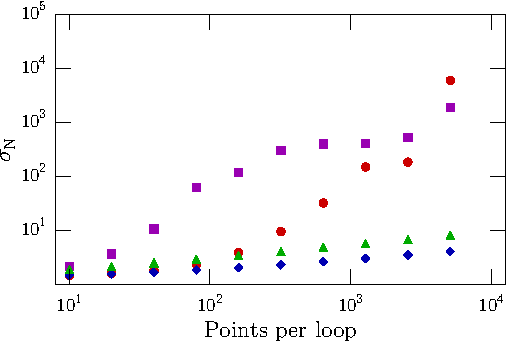
\includegraphics[width=0.8\textwidth]{fig/temp/TM_scalingN}
  \caption[Scaling of variance TM potential as function of $N$ for four methods.]
  {Scaling of variance TM potential as function of $N$ for four methods.  
  All combinations of Gaussian paths increments and combined TM-Gaussian steps, with raw values and 
  birth-death.}
\label{fig:TM_scalingN}
\end{figure}

Fig.~\ref{fig:TM_scalingN} shows how the Gaussian and TM-Gaussians estimates of the simple path integral
scale with the path resolution.  The birth-death process has been applied to both ways of generating paths.
The birth-death process reduces the variance, and makes both methods much more tractable.
The difference between Gaussian and TM-gaussians is small under the birth-death process.
Given that small difference, and the relative simplicity of the Gaussians, we have opted to 
use the birth-death process in conjunction with Gaussians throughout the remainder. 

\subsection{Monte-Carlo Sampling for Path-Time}

\label{sec:expT-sampling}

The TM polarization requires a slightly different sampling method for generating path-times $\cT$.  
In some limited cases it may be possible to estimate a minimum $\cT_0$ where 
the integrand is small for a given path, and a path is unlikely to have branched or birthed new paths.  
For paths starting on the vacuum side near a dielectric, the accumulated
potential at small path-times is approximately ${\prod_k( 1+\tanh\Xi e^{-2(d-x_k)(d-x_{k+1})/\Delta\cT})}$,  
which turns on smoothly in $\cT$.
In that case, $\cT_0$ can be estimated from the time an initial, fiducial path would contact a surface and the 
integrand would turn on.  The path-time can be sampled from the power law distribution~(\ref{eq:Tpower_law}).
The birth-death process then proceeds starting with the initial path.  

However, in a two-body geometry that sort of estimation fails.
The renormalized integrand is only nonzero for paths that come close to both surfaces.
Since the birth-death method may split the trajectory, it is not always possible to reliably
find a minimum time $\cT_0$ when the renormalized integrand turns on.  (A very small $\cT_0$ could be picked, 
where the path has no chance of touching the surface, but most computations would return zero,
 since the most probable $\cT$ are close to $\cT_0$.)
As a result, it is not possible to estimate for a single trajectory a lower bound $\cT_0$ 
for which the path does not branch, but is also close to when the integrand turns on.  

Since the birth-death method essentially enlarges the ensemble of paths selected, it's turn on
closely mimics the probability for a Brownian bridge to touch a surface.
The probability for a Brownian bridge to touch a surface a distance $d$ away in path-time $\cT$ is 
\begin{equation}
  P_{\text{touch}}(\cT) = e^{-2d^2/\cT}.
\end{equation} 
The combined potential term ${\prod_kv_{k,k+1}}$,  also has a similar dependence.  
This could be combined with the $\cT^{-(1+D/2)}$ power law for a new probability distribution.  
\begin{equation}
  P_{\text{exp-T}}(\cT;\cT_0,s) = \frac{\cT_0^{s-1}}{\Gamma[s-1] \cT^s}e^{-\cT_0/\cT}\label{eq:expT},
\end{equation}
where $s>1$ and $\cT_0>0$.  
%  The exponential factor effectively models the finite touching 
% probability for Brownian bridges starting at the origin to touch a planar surface a distance $d$ 
% away in time $\cT$, $P_\text{touch}=e^{-2d^2/\cT}$. 
The probability distribution~\ref{eq:expT} can be transformed to $u=\cT_0/\cT$, for 
which the probability distribution is
\begin{equation}
  P_{\text{exp}-1/\cT}(u;s) = \frac{u^{s-2}}{\Gamma[s-1]}e^{-u}.
\end{equation}
% where we had to include $du/d\cT= -(\cT_0)/\cT^2=-1/(\cT_0u^2)$ for the change
% of measure.  
The new variable $u=\cT_0/\cT$ has the form of a Gamma distribution, which has probability density 
\begin{equation}
  f(x) = \frac{x^{a-1} e^{-x/b}}{\Gamma(a)b^a}.  
\end{equation}
where $a>0$ and $b>0$ are the shape and scale parameters respectively~\cite{Devroye2003}.  
For small integer or half-integer powers $a$, there are some simple methods for generating 
gamma deviates $g_i$.  
A sum of Gamma deviates $\sum_{i=1}g_i$ with shape parameters $a_i$, is also a Gamma deviate
with shape parameter $\sum a_i$~(see pg. 402 of Devroye~\cite{Devroye2003}).  
In particular, this means the sum of $k$ exponential deviates $e_i=-\log(u_i)$, yields a Gamma 
deviate gamma(k,1).  Furthermore if $z$ is normally distributed then $z^2/2$ obeys gamma$\left(\frac{1}{2},1\right)$.
For small integer powers, $\cT$ is distributed according to
\begin{equation}
  \cT\sim \frac{\cT_0}{-\sum_{i=1}^{s}\log u_i},
\end{equation}
while for half-integer powers, 
\begin{equation}
  \cT\sim \frac{\cT_0}{-\sum_{i=1}^{\text{floor}(s)}\log u_i+z^2/2}.
\end{equation}
The integer powers are useful for estimating zero temperature Casimir energies. The half-integer powers
naturally emerge when considering the thermal Casimir energy, or derivatives of the Casimir energy 
such as the force.  
This distribution can also be used to sample times $\cT$
even for TE integrands.  In that case however, it is possible the generated path will not
touch all bodies and merely return zero.    


\subsection{Gradient Estimation}

Computing the TM Casimir--Polder energy~\ref{eq:TM_Casimir_Polder}, requires taking two spatial derivatives
of the worldline path integral.
Furthmore, in some experiments on the Casimir--Polder effect such as BEC experiments~\cite{Harber2005}, 
the Casimir--Polder potential is estimated from how it shifts the frequency of the atom's oscillations
in a harmonic potential.  This frequency shift is calculated by taking two derivatives of the Casimir--Polder
potential.   For the TM polarization within the worldline method, this would require four spatial 
derivatives, so it is essential to be able to efficiently compute these derivatives.  

Consider a generic worldline path integral involving pinned Brownian motions in path-time $\cT$ with starting point $\vect{x}_0$
\begin{equation}
  I(x_0)=\dlangle \Phi(x_0,x_1,\ldots,x_{N-1})\drangle_{\vect{x}(t),\vect{x}(0)=\x0}.
\end{equation}
The function $\Phi$ depends on the whole path, and serves as a placeholder for the path-averaged dielectric
or TM potentials.  The $n^\text{th}$ derivative of this path integral with respect to the starting
position is 
\begin{equation}
  \partial_0^nI(x_0)=\frac{\partial^n}{\partial x_0^n}\dlangle \Phi\drangle_{\vect{x}(t),\vect{x}(0)=\x0}.
\end{equation}
We will discuss how to evaluate this derivative with both the finite difference method 
and the partial-averaging approach.

\subsection{Finite Differences}

The finite difference method is simplest method for numerically evaluating derivatives.
 It has the great virtue of simplicity, since it only requires that we evaluate the function multiple times.  
For smooth functions, the finite difference method works well, but it behaves poorly when applied to
stochastic, discontinuous functions such as the worldline path integral. 

For example, consider the first derivative of the TE Casimir--Polder worldline integrand,
at a dielectric step $\epsr=1+\chi\Theta(x-d)$.  The finite difference integrand is
\begin{equation}
  \partial_0\Bigdlangle \,\langle\epsr[\vect{x}(t)\rangle^{-3/2}-1\Bigdrangle_{\vect{B}_k}
  = \frac{1}{\Delta s}\Bigdlangle \, \langle\epsr[\vect{x}_0+\Delta s\hat{r}_i+\sqrt{\cT}B_k]\rangle^{-3/2}
  -\langle\epsr[\vect{x}_0+\sqrt{\cT}B_k]\rangle^{-3/2}\,\Bigdrangle_{\vect{B}_k}
\end{equation}
where $\Delta s$ is the finite difference step size, $\vect{B}_k$ is a closed unit Brownian bridge, 
and $\hat{r}_i$ is a Cartesian unit vector.
This can be evaluated on a path-wise basis.  
In order to be accurate, the step size $\Delta s$ must be small, since the error in this approximation 
to the derivative is $\order[(\Delta s)^2]$.
Unfortunately, that limit leads to large fluctuations.
If the finite difference is much smaller than a typical path increment,$\Delta s\ll \sqrt{\Delta\cT}$, 
the estimates for path-averaged dielectirc $\langle\epsr(\vect{x}_0)\rangle$ for the two starting positions
are likely to be the same, so the estimate is zero.  
In rare circumstates, a point is within $\Delta s$ of the surface, and the finite difference returns
the large value of $(\Delta s)^{-1}$.
Thus most paths estimate zero derivative, but a few paths return a large answer.  This leads to 
growing fluctations.  This problem is even worse for higher derivatives.  
%In evaluating the finite difference it is best to use the same random numbers to generate the path~\cite{Asmussen2008,Glasserman2004}.

The finite difference method is also problematic for the birth-death method for TM potentials.  
In that case, as the starting position of the paths varies, a different family
of birth-death paths may be generated, which further compounds the fluctuation problem.    

% We should note that in planar geometries, the integration over $\cT$ can remove this problem
% for TE integrands.  In that case, the path integral changes value whenever a path point $x_k$ 
% enters a surface at $x=d$.  

% \begin{enumerate}
%   \item Best to use common random numbers.  Also provides better error estimate.
%   \item Need to balance choosing $N$, $ds$.  
%   \item However difference-of-ensembles has better behaviour than 
%     ensemble-of-differences.  Some ordering of operations noticeably superior.  
%     Essentially passes finite difference onto $1/\cT^3$, which is nice and smooth.
% \end{enumerate}

\subsection{Malliavin Calculus}
Similar derivatives are required in quantitative finance, where the sensitivity of a financial 
product to variations its underlying parameters must be estimated.  This could be done via a finite
difference method, but that behaves poorly.  
Since financial simulations also typically involved averages over simulated Brownian motions, similar problems emerge.
One promising approach for worldline applications is based on the Malliavin calculus, which 
is formally discussed in Ref.~\cite{Nualart2006, Malliavin2006, DiNunno2009}.
Less formal (and more understandable) discussions of the Malliavin approach are presented in Refs.~\cite{Chen2007,Kohatsu-Higa2003}.
In the Malliavin approach, the derivative can be estimated by \emph{multiplying} the integrand by
a suitably chosen weight function, which depends on the nature of the derivative and the random path.
The Malliavin calculus is essentially functional differentiation with respect to the Brownian motion, 
and an associated integration by parts formula.   
The Malliavin weights can be derived by exchanging derivatives with respect to a parameter for
derivatives with respect to the Brownian motion, and integrating by parts~\cite{Kohatsu-Higa2004}.  
The Malliavin results can also be recovered via the likelihood-ratio method\footnote{
In the likelihood ratio method~\cite{Broadie1996}, a derivative with respect to a parameter $\theta$ of a stochastic average is evaluated 
as $\partial_\theta\dlangle \Phi(x)\drangle = \int dx\,\Phi(x)\partial_\theta P(x,\theta) 
= \dlangle \Phi(x)\partial_\theta\log P(x,\theta)\drangle$,
where $\partial_\theta\log P$ is the likelihood function.  
The original sampling method can be used to evaluate this derivative, so $\dlangle\Phi\drangle$ and its derivatives
$\partial_\theta\dlangle \Phi\drangle$ can be evaluated using the same random samples.}
in conjunction with partial-averaging along the Brownian motion~\cite{Chen2007}. 
In either case, one exchanges differentiation for
evaluating a new reweighted function, which depends on the required derivatives, while still
using the original paths.  

While the Malliavin approach to derivative estimation did not yield better results for the worldline
method, it did inspire a similar approach, with similar virtues.   

\subsection{Partial Averaging Gaussian Paths}

\label{sec:partial_average}
Let us consider the derivative of 


    Momentarily focus on just the path integral piece,
    \begin{equation}
      P = \biggdlangle e^{-s\cT \langle \epsr\rangle}\biggdrangle 
      = \int \prod_{j=1}^{N-1}dx_k \prod_{j=0}^{N-1}\frac{1}{(2\pi \Delta T)^{D/2}}e^{-(\vect{x}_{j+1}-\vect{x}_j)^2/2\Delta T-s\Delta T \epsr(\vect{x}_j)}.
    \end{equation}
    Main component are derivatives w.r.t. Gaussian.  


    Our basic idea is to integrate out intermediate coordinates.  Under the assumption the 
    the integrands are approximately stable, or that the steps compose, we can average multiple
   %  steps.
   % This is related to choosing a non-uniform loop with less resolution close to the beginning of the 
   %  loop.  This is justified via switching integration and differentation.  The Gaussian integrals 
   %  obviously compose.  The derivatives can just be carried out at the very end.  

   Derivatives of the Gaussian are Hermite polynomials:
    \begin{equation}
      \frac{d^n}{dx^n} e^{-x^2} = (-1)^n H_n(x)e^{-x^2}
    \end{equation}
    Scaling the variables to $x\rightarrow x/a$ yields
    \begin{equation}
      \frac{d^n}{dx^n} e^{-(x-\mu)^2/a^2} = a^{-n}(-1)^n H_n\big(\frac{x-\mu}{a}\big)e^{-(x-\mu)^2/a^2}
    \end{equation}

    The simplest approach is to exchange integration and differentiation, then completing the square in $x_0$,
    and then carry out the derivatives
    \begin{align}
      C=&\partial_0^n\int dx_1  \frac{1}{(2\pi)^{3/2}\sqrt{T_1T_2T_{N_1}}}e^{-(x_0-x_1)^2/(2T_1)-(x_1-x_2)^2/(2T_2)-(x_0-x_{N-1})^2/(2T_{N-1})}\\
%      =&\partial_0^n \frac{1}{2\pi\sqrt{(T_1+T_2)T_{N_1}}}e^{-(x_0-x_2)^2/[2(T_1+T_2)]-(x_0-x_{N-1})^2/(2T_{N-1})}\\
      =&\partial_0^n \frac{1}{2\pi\sqrt{(T_1+T_2)T_{N_1}}}e^{-(x_0-\mu_2)^2/[2\sigma_2^2]-(x_2-x_{N-1})^2/(2[T_{N-1}+T_1+T_2])}\\
      =&(-1)^n(\sqrt{2}\sigma_2)^{-n/2}H_n\bigg(\frac{x_0-\mu_2}{\sqrt{2}\sigma_2}\bigg)
      \frac{1}{(2\pi)\sqrt{(T_1+T_2)T_{N_1}}}\nonumber\\
      &\times e^{-(x_0-x_2)^2/[2(T_1+T_2)]-(x_0-x_{N-1})^2/(2T_{N-1})},
    \end{align}
    where 
    \begin{gather}
      \mu_2 = \frac{T_{N-1}x_2+ (T_1+T_2)x_{N-1}}{T_1+T_2+T_{N-1}}\\
      \sigma_2^2 = \frac{(T_1+T_2)T_{N-1}}{T_{N-1}+T_1+T_2}
    \end{gather}

 Now evidently if we integrate out points symmetrically from the loop origin, and we 
    assume all $T_i=\Delta T$, then after integrated out $m$ steps we have 
    \begin{gather}
      \bar{x}_m = \frac{x_{m+1}+ x_{N-m-1}}{2}\\
      \sigma_2^2 = m\Delta T.
    \end{gather}
    The gradient of the path integral can then be approximately written as 
    \begin{align}
      C\approx
      &(-1)^n(\sqrt{2 T_m})^{-n/2}H_n\bigg(\frac{x_0-\bar{x}_m}{\sqrt{2 T_m}}\bigg)\nonumber\\
      &\times \frac{1}{(2\pi T_m)}e^{-(x_0-x_{m+1})^2/(2T_m)-(x_0-x_{N-m-1})^2/(2T_m)}.
    \end{align}

 We can estimate how many steps to integrate out based on the touching probability in time $T_m$.  
    The probability to touch a plane a distance $d$ away in time $T_m=m\Delta T = (m/N)T$ is 
    \begin{equation}
      P_{\text{touch}} = e^{-2d^2/T_m},
    \end{equation}
    which can be solved for $m$ if we require that $P_{\mathrm{touch}}$ does not exceed a threshold
    $10^{-\rho}$ with $\rho>0$  
    \begin{equation}
      \frac{m}{N} \le \frac{2d^2}{T\rho\ln(10)}.
    \end{equation}
    Note that as $N$ increases, the integration point approaches a constant fraction, even as $N$ increases.  
    This in effect reduces the fluctuations by $m^n$.  
  
 This is in effect choosing to make a loop with non-uniform steps, where in particular the first
    and last step are larger than the others.  We choose the size of those steps to be as 
    large as possible, while not interacting much with a the nearest surface.  

 Problem with adaptive choice?


\subsection{General Method Near Surfaces}

     While estimating gradients for the stress-tensor it may be necessary to estimate 
    gradients while close to one surface.  For a renormalized energy, only loops that touch both
    surfaces will contribute.   In this case, the above approach based on integrating out Gaussians
    is of limited utility in reducing the fluctuations.  The assumption that the integrals are approximately
    Gaussian can only be explited for a very small number of steps.  
    However, if we assume there is a Feynman-Kac formula available taking into account the 
    interaction with a simple surface, then similar reasoning can be used.  In this case
    one integrates out further steps, since the Feynman-Kac formulae compose with one another,
    where now the threshold is must balance the path wandering sufficiently far that a simple 
    approximation.

    For example, consider using the Feynman-Kac formula for open loops near a Dirichlet surface, 
    \begin{equation}
      \dlangle e^{-V_D(x-d)}\drangle_{x_{j}\rightarrow x_{j+1}} 
      = \Theta[(x_j-d)(x_{j+1}-d)]\left(1-e^{-2(x_j-d)(x_{j+1}-d)/T}\right)
    \end{equation}

\begin{enumerate}
  \item Gradients for atom
  \item Stress energy tensor 
\item Application to stress-tensor.  (Evaluate derivatives first, then take limit.)
  Problematic for stress-tensor values near one surface in 2-body scenarios. (Use exponential expressions
  to allow non-Gaussian integration.  Must just be stable distribution  
  Thus expact larger fluctuations near surfaces.  
  For example, stress-energy tensor requires 
  \begin{equation}
   T_{zz}=\lim_{\Delta\rightarrow 0} [\partial_{x_{CP}}^2 - \partial_{\Delta}^2]\dlangle \mathfrak{M}\drangle,
  \end{equation}
  where $\Delta = (x_N-x_0)/2, x_{CP} = (x_N+x_0)/2$.  Using the chain-rule, and employing the
  same differentiation this becomes. where $x_{CP}$ is the centre-point, and $\Delta$ is the separation.
%   \begin{gather}
%     x_{CP} =  \frac{1}{2}(x_{N}+x_0)\\
%     \Delta = \frac{1}{2}(x_{N}-x_0)\\
%     x_0  = x_{CP}-\Delta\\
%     x_N = x_{CP}+\Delta
%   \end{gather}
%   Then
%   \begin{align}
%     \frac{\partial}{\partial x_{CP}} 
%     %&= \frac{\partial x_0}{\partial x_{CP}}\frac{\partial}{\partial x_0}
%     % +\frac{\partial x_N}{\partial x_{CP}}\frac{\partial}{\partial x_N}\\
% &= \frac{1}{2}\frac{\partial}{\partial x_N}+\frac{1}{2}\frac{\partial}{\partial x_0}\\
%   \frac{\partial}{\partial \Delta} 
% %&= \frac{\partial x_0}{\partial \Delta }\frac{\partial}{\partial x_0}
% %    +\frac{\partial x_N}{\partial \Delta}\frac{\partial}{\partial x_N}\\
% &= \frac{1}{2}\frac{\partial}{\partial x_N}-\frac{1}{2}\frac{\partial}{\partial x_0}
%   \end{align}
Then expanding these derivatives out (correct expression?)
\begin{align}
  T_{zz} &= \lim_{x_N\rightarrow x_0}\frac{1}{4}[(\partial_0+\partial_N)^2+(\partial_0+\partial_N)^2]G\\
  &= \lim_{x_N\rightarrow x_0}\frac{1}{2}[\partial_0^2+\partial_N^2]G
\end{align}

\end{enumerate}

\subsection{Hermite-Gaussian Sampling}

In order to apply the Hermite-Gaussian method to high order derivatives, it is best to 
sample from the combined Hermite-Gaussian.  The simplest approach uses Gaussian samples, weighted
by the appropriate Hermite-Gaussian function.  While this is acceptable for the first or second derivatives,
it breaks down for higher derivatives.  In particular, the Gaussian samples are most likely to be in a narrow
range $x\in(-3\sigma,3\sigma)$.  The Hermite-Gaussian oscillates in sign in this range, and
the dominant contributions come from the tails $x\sim \sqrt{n}\sigma$.  So for a finite sample,
one would see large fluctuations.  

The combined Gaussian steps for both $x_1, x_2$ which are pinned to start at $x_0$ is 
\begin{align}
  G &= \frac{1}{2\pi T_1T_2}\exp\left[-\frac{(x_0-x_1)^2}{2T_1}-\frac{(x_0-x_2)^2}{2T_2}\right]\\
  % &= \frac{1}{2\pi T_1T_2}\exp\left[-\frac{T_1+T_2}{2T_1T_2}x_0^2 +\left(\frac{x_1}{T_1}+\frac{x_2}{T_2}\right)x_0
  %   -\frac{x_1^2}{2T_1}-\frac{x_2^2}{2T_2}\right]\\
  &= \frac{1}{2\pi T_1T_2}\exp\left[-\frac{T_1+T_2}{2T_1T_2}\left(x_0 -\frac{x_1T_2+T_1x_2}{T_1+T_2}\right)^2
    -\frac{(x_1-x_2)^2}{2(T_1+T_2)}\right]
\end{align}
After differentiation w.r.t $x_0$, one finds 
\begin{equation}
  HG:= \partial_0^n G 
= \frac{1}{\sqrt{2\pi\sigma^2}\sqrt{2\pi(T_1+T_2)}} 
(-1)^n(2\sigma^2)^{-n/2}H_n\left(\frac{x_0-\mu_H}{\sqrt{2\sigma_H^2}} \right)
  \exp\left[-\frac{(x_0-\mu_H)^2}{2\sigma_H^2} - \frac{(x_1-x_2)^2}{2(T_1+T_2)}\right],
\end{equation}
where 
\begin{gather}
  \sigma_H^2:= \frac{T_1T_2}{(T_1+T_2)}\qquad
  \mu_H := \frac{x_1T_2+T_1x_2}{T_1+T_2}.
\end{gather}
In the event that $T_1=T_2$, this simplifies down to 
\begin{gather}
  \sigma_H^2:= \frac{T_1}{2}\qquad
  \mu_H := \frac{x_1+x_2}{2}.
\end{gather}
In order to make samples that are useful for closed paths one must include 
the normalization factor for the ``open'' Gaussian bridge that connects the end points $x_1$ and $x_2$
in time $T-T_1-T_2$.  
The total distribution for $x_1,x_2$ is 
\begin{align}
  HG'(x_1,x_2)&:=\frac{1}{\sqrt{2\pi\sigma^2}\sqrt{2\pi(T_1+T_2)}\sqrt{2\pi(T-T_1-T_2)} }
  (2\sigma^2)^{-n/2}H_n\left(\frac{x_0-\mu}{\sqrt{2\sigma^2}} \right)\nonumber\\
  &\hspace{0.5cm}\times\exp\left[-\frac{(x_0-\mu)^2}{2\sigma^2} - \frac{T(x_1-x_2)^2}{2(T-T_1-T_2)(T_1+T_2)}\right],
\end{align}
However, this is not normalized, and can even change sign.  
The samples must be taken from the absolute value of the integrand, with the sign of the Hermite-Gaussian
function weighting the samples.
The sign changes will naturally lead to cancellation.  In the presence of a potential $\Phi[x(t)]$,
the cancellation is not perfect and the result is non-zero.  
In order to best carry out the cancellation, and reduce fluctuations one should pair each sample of 
the Hermite-Gaussian with its negative.  

The probability distribution for the combined steps can be most naturally formulated in terms of the decoupled variables
\begin{align}
  \bar{x}:=\frac{x_1+x_2}{2}\\
  \Delta x := x_2-x_1.
\end{align}
The probability distributions for $\bar{x}$ and $\Delta x$ decouple as 
\begin{align}
  P_{HG,1}(\bar{x})&:=\frac{1}{\sqrt{2\pi\sigma_H^2}} 
  \bigg|H_n\bigg(\frac{x_0-\bar{x}}{\sqrt{2\sigma_H^2}} \bigg)\bigg|
  %\nonumber\\  &\hspace{0.5cm}\times
  \exp\left[-\frac{(x_0-\bar{x})^2}{2\sigma_H^2}\right]\\
  P_{HG,2}(\Delta x) &:=\sqrt{\frac{T}{2\pi(T_1+T_2)(T-T_1-T_2)}}
%  &\hspace{0.5cm}\times
\exp\left[- \frac{T(x_1-x_2)^2}{2(T-T_1-T_2)(T_1+T_2)}\right],
\end{align}
The numerical average can be computed as 
\begin{equation}
  I = \dlangle (-1)^n(2\sigma_H^2)^{-n/2}\eta_Hs_Hf\drangle_{HG},
\end{equation}
where $x_1,x_2$ are sampled from $P_{HG}$, and the remaining sub-bridge is sampled via
the open Gaussian probability distribution.  
where the normalization $\eta_H$ and sign factor $s_H$ are defined as 
\begin{align}
  s_H &:= \sgn\bigg[H_n\left(\frac{x_0-\mu_H}{\sqrt{2\sigma_H^2}} \right)\bigg] \\
  \eta_H &:=\frac{1}{\sqrt{2\pi T}}\int dy \frac{1}{\sqrt{2\pi\sigma_H^2}}
  \big|H_n\left(\frac{x_0-y}{\sqrt{2\sigma_H^2}} \right)\big|
%  \nonumber\\  &\hspace{0.5cm}\times
\exp\left[-\frac{(x_0-y)^2}{2\sigma_H^2}\right],
\end{align}

It is best to numerically sample from distributions with unit variance, and rescale the deviates 
by the time.  In which case, $\bar{x}=h\sqrt{2\sigma_H}$, and $\Delta x = \sqrt{2T_1(T-2T_1)/T}z$,
where $z$ is a standard normal deviate as $h$ is sampled from 
\begin{align}
  P'_{HG,1}(h)&:=\frac{1}{\eta'_H\sqrt{\pi} }  \bigg|H_n\bigg(-h\bigg)\bigg|e^{-h^2}\\
  \eta'_H&=:=\int dh P'_{HG,1}(h).
\end{align}

The raw deviates will be denoted $h$ and $z$.% , where 
% \begin{align}
%   \frac{1}{2}(x_1+x_2) &= x_0 + \sqrt{\frac{T_1}{2}}h\\
%   -x_1+x_2 &= \sqrt{\frac{2T_1(T-2T_1)}{T}}z
% \end{align}
Then solving for $x_1, x_2$, 
\begin{align}
  x_1 & = x_0 + \left(\sqrt{\frac{T_1}{2}}h-\sqrt{\frac{T_1(T-2T_1)}{2T}}z\right)\\
  x_2 & = x_0 + \left(\sqrt{\frac{T_1}{2}}h+\sqrt{\frac{T_1(T-2T_1)}{2T}}z\right)
\end{align}
where $h' := h\sqrt{T_1/2}, z' := z\sqrt{\frac{T_1(T-2T_1)}{2T}}$.
\comment{Note these variables are scaled to agree with Dan, whose code seems to output 
  $h/\sqrt{2}$ naturally.  Again, he is treating $H_n(x)e^{-x^2}$ as the probability
  distribution.}






\subsection{TM Numerical Results: Planar Casimir Energies}


\begin{figure}
\centering
  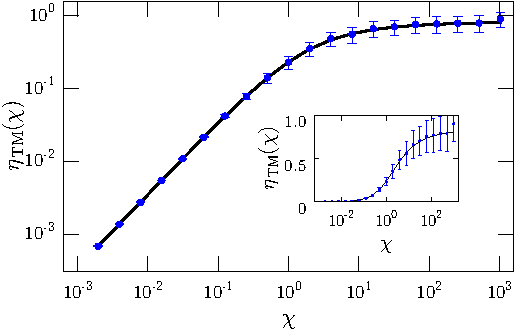
\includegraphics[width=0.8\textwidth]{fig/temp/eff_TM_atom_wall}
  \caption{Numericall computed TM Casimir--Polder Efficiency for Atom-Plane.  }
\end{figure}

\begin{figure}
\centering
  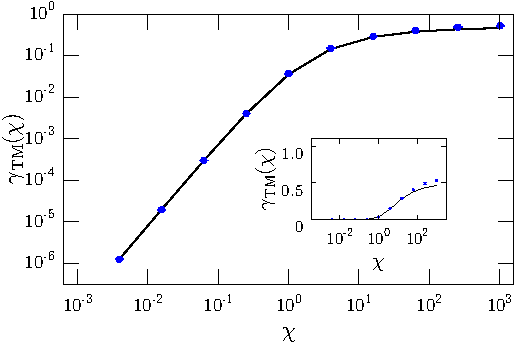
\includegraphics[width=0.8\textwidth]{fig/temp/eff_TM_2wall}
  \caption{Numericall computed TM Casimir Efficiency for Plane-Plane.  }
\end{figure}


\subsection{Path Construction Revisited: Path-Pinning as Importance Sampling}

In the curvature numerics, the forces emerged from paths constrained to touch the surfaces 
of the interacting bodies.  While this is a necessity for forces, constrained paths can also be used
to compute Casimir energies.
Although the Casimir energies do not require such constraints, the renormalized 
integrand is only non-zero for paths that touch both surfaces.
This suggest using paths constrained to touch both surfaces by construction.  This is a form of importance
sampling, beyond what is suggested by the Gaussian measure of the worldline path integral.
We would construct paths that are constrained to touch both surfaces, and correct for this modification
to the path integral.  In the TM Casimir energy, this is very useful, since the birth-death method 
causes many paths to be created, and ideally most of these new paths would also contribute to the path 
integral.  
In the absence of such a bias, a large number of paths are created near one surface, and if these paths
do not intersect the other body, a large amount of computational effort is wasted.  

Consider a Gaussian path integral,
\begin{equation}
  I_k=\int \frac{d\cT}{(2\pi)^{D/2}\cT^{1+D/2}}\int d\vect{x}\, f(\vect{x})P(\vect{x}),
\end{equation}
where $f$ is some function of the whole path that is only non-zero if the path enters a given region.
The $D-1$-dimensional probability density is given by,
\begin{equation}
  P(\{\vect{x}\}) = (2\pi\cT)^{(D-1)/2}\prod_{k=0}^{N-1} \frac{1}{(2\pi\Delta\cT)^{(D-1)/2}}e^{-(\vect{x}_{k+1}-\vect{x}_k)^2/(2\Delta\cT)},
\end{equation}
Instead of just taking $P$ as the probability density, let us consider using $Q=P(\vect{x})|_{x_k=d}$,
where one point is fixed on the surface of the region
\begin{align}
  Q(\{\vect{x}\}) =& (2\pi\cT)^{(D-1)/2}\cN_Q^{-1}\prod_{j=0}^{N-1}
 \frac{1}{(2\pi\Delta\cT)^{(D-1)/2}}e^{-(\vect{x}_{j+1}-\vect{x}_j)^2/(2\Delta\cT)}\bigg|_{x_k=\vect{d}},
  \end{align}
  where the normalization constant is
\begin{equation}
\cN_Q=\bigg[\frac{N^2}{2\pi k(N-k)\cT}\bigg]^{(D-1)/2}
e^{-N^2(\vect{d}-\vect{x}_0)^2/[2k(N-k)\cT]}
\end{equation}
The ratio of the probability densities is 
\begin{align}
  \frac{P}{Q} &= \cN_Q\frac{\exp\left[-\frac{(\vect{x}_{k-1}-\vect{x}_k)^2}{2\Delta \cT}
      -\frac{(\vect{x}_{k}-\vect{x}_{k+1})^2}{2\Delta \cT}\right]}
  {\exp\left[-\frac{(\vect{x}_{k-1}-\vect{d})^2}{2\Delta \cT}
      -\frac{(\vect{d}-\vect{x}_{k+1})^2}{2\Delta \cT}\right]}
%  \\  &
= \cN_Q\exp\left[-\frac{(\vect{x}_{k}-\bar{\vect{x}})^2}{\Delta \cT}
      +\frac{(\vect{d}-\bar{\vect{x}})^2}{\Delta \cT}\right].
\end{align}
% Note that the paths are constructed to ensure $\vect{x}_0\rightarrow\vect{d}$.  There is still one 
% remaining integral which can also be sampled from in determining the integrand, but this sampled $\vect{x}_k$
% does not alter the path.  

The resulting integrand could be built up from Monte Carlo samples 
\begin{equation}
  I_k = \int \frac{d\cT}{(2\pi)^{D/2}\cT^{1+D/2}}\int d\vect{x}_k\, \cN_Q e^{-\frac{(\vect{x}_{k}-\bar{\vect{x}})^2}{\Delta \cT}
      +\frac{(\vect{d}-\bar{\vect{x}})^2}{\Delta \cT}} f(\vect{x})Q(\vect{x})
\end{equation}
The normalization $\cN_Q$ can be used to sample the times, with $s=D/2$ and $\cT_0=N^2|\vect{d-x}_0|^2/[2k(N-k)]$ as the distribution
parameters.
The remaining $\vect{x}_k$ integral can be evaluated by using the Gaussian.
However, those sampled values of $\vect{x}_k$ are not the path values, rather they are sampled after
the path is constructed subject to the pinning requirement.    
The appropriate integrand for Monte carlo in pinned paths, $\vect{x}_k$ and times $\cT$ is 
\begin{align}
  I_k &= \dlangle \frac{\Gamma[D/2]}{\cT_0^{D/2}}\bigg(\frac{N}{2\pi k (N-k)\Delta\cT}\bigg)^{(D-1)/2}
  (\pi \Delta\cT)^{(D-1)/2} e^{\frac{(\vect{d}-\bar{\vect{x}})^2}{\Delta \cT}} f(\vect{x})\drangle_{\{\vect{x}\}',\vect{x}_k,\cT}\nonumber\\
   % &= \dlangle \Gamma[D/2] \left(\frac{2k(N-k)}{N^2\vect{|d-x_0|}^2}\right)^{D/2} \frac{N^{n/2}}{[2k(N-k)]^{n/2}}
   %  e^{\frac{(\vect{d}-\bar{\vect{x}})^2}{\Delta \cT}} f(\vect{x})\drangle_{\{\vect{x}\}',\vect{x}_k}\\
   &= \dlangle \Gamma[D/2] \frac{[2k(N-k)]^{(D-n)/2}}{N^{D-n/2}\vect{|d-x_0|}^D}   
   e^{\frac{(\vect{d}-\bar{\vect{x}})^2}{\Delta \cT}} f(\vect{x})\drangle_{\{\vect{x}\}',\vect{x}_k,\cT}.
 \end{align}

Of course, if the pinned point is also integrated over (such as the transverse dimensions for a planar medium),
 then a different distance dependence.
  In that case, only one dimension remains to be evaluated in the path integral,
% \begin{align}
%   I   &= \dlangle \Gamma[D/2] \frac{[2k(N-k)]^{(D-1)/2}}{N^{D-1/2}|d-x_0|^D}   
%   e^{\frac{(\vect{d}-\bar{\vect{x}})^2}{\Delta \cT}} f(\vect{x})\drangle_{\{\vect{x}\}',\vect{x}_k,\cT}.
% \end{align}
The result can be written out explicitly for $D=4$
\begin{align}
  I   &= \dlangle  \frac{[2k(N-k)]^{3/2}}{N^{2}N^{3/2}|d-x_0|^4}   
  e^{\frac{(\vect{d}-\bar{\vect{x}})^2}{\Delta \cT}} f(\vect{x})\drangle_{\{\vect{x}\}',\vect{x}_k,\cT}.
\end{align}

The above development fixed one particular index $k$.  This index $k$ can also be sampled over to vary
which points are pinned to the surface.  We propose using $P_k= 6 k(N-k)/N^2$, as this is simple to sample
from and is not too sharpled peaked around $k=N/2$.
\comment{need to integrate over surface, changes normalization, changes dimension of normalization $\implies$
  leftover $k$ dependence}

% The normalization for path subject to a single constraint is 
% \begin{equation}
%   \mathcal{N}_1=\mathcal{G}\big[\vect{x}_0,\vect{d},k(N-k)\cT/N^2\big],
% \end{equation}
% exactly as emerged for the potential curvature.  We will use this to sample times
% as described in Sec.~\ref{sec:expT-sampling}.

% The normalization for the $Q$ probability distribution is 
% \begin{equation}
%   \cN =\frac{1}{[2\pi k \Delta \cT]^{D/2}[2\pi (N-k)\Delta \cT]^{D/2}}
%     e^{-N^2(\vect{x}_0-\vect{d})^2/(2k(N-k) \cT)}
% \end{equation}
% (a factor of $[2\pi\cT]^{D/2}$ mutliplies this if that is factored out for the usual Brownian bridge
% normalization).  This is the probability we must factor out to sample bridges for where the $k^{\text{th}}$ point
% is fixed.  
% Use that as basis to sample times, and indices.






%%% Local Variables: 
%%% mode: latex
%%% TeX-master: "thesis_master"
%%% End: 
